\documentclass[aspectratio=169]{beamer}
\PassOptionsToPackage{english}{babel}
\usepackage{standardslides}

\usepackage{tikz}
\usepackage{pifont}
\usepackage{listings}
\usepackage{colortbl}
\newlength{\listingframemargin}
\setlength{\listingframemargin}{1em}
\newlength{\listingmargin}
\setlength{\listingmargin}{0.08\textwidth}

\definecolor{codeDarkGray}{gray}{0.2}
\definecolor{codeGray}{gray}{0.4}
\definecolor{codeLightGray}{rgb}{0.94,0.94,0.91}
\definecolor{codeBorder}{rgb}{0.34,0.24,0.21}
\definecolor{MidnightBlue}{rgb}{0.1, 0.1, 0.8}

\lstdefinestyle{standard}{%
  belowcaptionskip=0.5\baselineskip,
  breaklines=true,
  frameround=tttt,
  % frame=false,
  xleftmargin=0em,
  xrightmargin=0em,
  showstringspaces=false,
  showtabs=false,
  % tab=\smash{\rule[-.2\baselineskip]{.4pt}{\baselineskip}\kern.5em},
  basicstyle= \fontfamily{pcr}\selectfont\scriptsize\bfseries,
  keywordstyle= \bfseries\color{MidnightBlue}, %\color{codeDarkGray},
  commentstyle= \itshape\color{codeGray},
  identifierstyle=\color{codeDarkGray},
  stringstyle=\color{BurntOrange}, %\color{codeDarkGray},
  numberstyle=\tiny\ttfamily,
  % numbers=left,
  numbersep = 1em,
  % stepnumber = 1,
  % captionpos=t,
  tabsize=2,
  % backgroundcolor=\color{codebLightGray},
  rulecolor=\color{codeBorder},
  framexleftmargin=\listingframemargin,
  framexrightmargin=\listingframemargin
}

\newcommand{\inputCodeBlock}[1]{%
  % \begin{mybox}
    \begin{center}
      % \begin{minipage}[c]{0.7\textwidth}
        \lstinputlisting[%
          style = standard,
          language = c++,
          morekeywords={constexpr,noexcept,decltype,size_t,uint32_t,uint64_t,__m256i,__m256,__m256d,__m128i,__m128,__m128d}
        ]{#1}
      % \end{minipage}
    \end{center}
  % \end{mybox}
}

\def\UrlBigBreaks{\do\/\do-\do:}

\title{%
  Design and Implementation of Vectorized Pseudorandom Number Generators%
  %and their Application to Simulations of Photon Propagation
}
\subtitle{Master's Thesis Defense and Presentation}
\author{Markus Pawellek}

\begin{document}
  \selectlanguage{english}
  % \urlstyle{sf}

  { % all template changes are local to this group.
      \setbeamertemplate{navigation symbols}{}
      \begin{frame}<article:0>[plain]
          \begin{tikzpicture}[remember picture,overlay]
              \node[at=(current page.center)] {
                  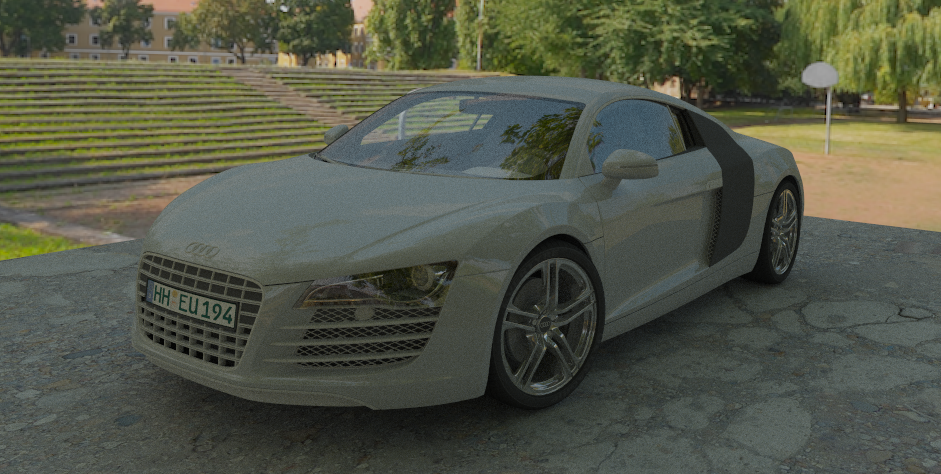
\includegraphics[keepaspectratio,
                                   width=1.2\paperwidth,
                                   height=\paperheight]{images/audi_r8_path_tracing_2.png}
              };
          \end{tikzpicture}
       \end{frame}
  }

  \frame{\titlepage}
  \begin{frame}{Outline}
    \footnotesize
    \hfill\parbox[t][7cm][l]{0.9\textwidth}{\tableofcontents}
  \end{frame}

  \section{Introduction} % (fold)
  \label{sec:introduction}
    \begin{frame}{Introduction}
      What do we need random numbers for?
      \pause
      \begin{itemize}
        \item Physical Simulations, based on Monte-Carlo Methods
      \end{itemize}
      \bigskip
      \pause
      Goals:
      \begin{itemize}
        \pause
        \item vectorize existing PRNGs
        \pause
        \item create a software library and design a good API
        \pause
        \item apply library to physical problems
        \pause
        \item compare performance to other implementations
      \end{itemize}
    \end{frame}

    % \begin{frame}{Preliminaries}
    %   \begin{itemize}
    %     \item not all motivational questions can be answered here in the introduction
    %     \item no c++ code shown
    %     \item why c++
    %     \item only two generators
    %     \item a few things will not be shown
    %     \item no theory shown why prngs good
    %   \end{itemize}
    % \end{frame}
  % section introduction (end)

  \section{Pseudorandom Number Generators} % (fold)
  \label{sec:pseudorandom_number_generators}
    \begin{frame}{True Randomness}
      What is a random sequence?
      \pause
      \begin{itemize}
        \item existing formal concepts not applicable to computer systems
        \pause
        % \item infinite sequence of numbers that cannot be generated by a computer
        \item nondeterministic, noncomputable, unpredictable
        \pause
        \item generated by hardware components based on chaotic processes
      \end{itemize}
      \bigskip
      \pause
      Disadvantages:
      \pause
      \begin{itemize}
        \item Unreproducibility
        \pause
        \item Speed Limitations
      \end{itemize}
    \end{frame}

    \begin{frame}{Pseudorandom Number Generator Definition}
      \begin{minipage}[c]{0.49\textwidth}
        \begin{figure}
          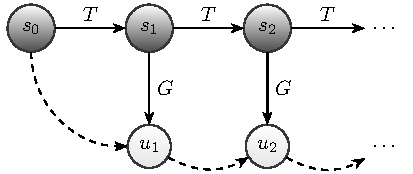
\includegraphics[width=\textwidth]{figures/sequence_generation_scheme.pdf}
        \end{figure}
      \end{minipage}
      \begin{minipage}[c]{0.49\textwidth}
        \begin{align*}
          &S\ldots\text{Set of States}\\
          &T\ldots\text{Transition Function} \\
          &U\ldots\text{Set of Possible Outputs} \\
          &G\ldots\text{Generator Function}
        \end{align*}
      \end{minipage}
      \vfill
      \begin{mybox}
        \[
          \mathscr{G} \define (S,T,U,G),\qquad \function{T}{S}{S}, \qquad \function{G}{S}{U}
        \]
        \[
          s_0\in S, \qquad s_{n+1} \define T(s_n), \qquad u_n \define G(s_n)
        \]
      \end{mybox}
    \end{frame}
  % section pseudorandom_number_generators (end)

  \section{Design of pXart} % (fold)
  \label{sec:design}
    % \begin{frame}{Design Components}
    %   \begin{figure}
    %     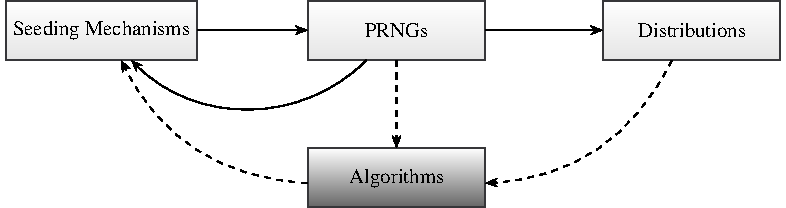
\includegraphics[width=\textwidth]{figures/api_parts.pdf}
    %   \end{figure}
    %   \begin{itemize}
    %     \pause\item pXart: header-only library written in C++
    %     \pause\item support for CMake and build2
    %     \pause\item providing online documentation
    %   \end{itemize}
    % \end{frame}

    \begin{frame}{Design Components}
      \begin{figure}
        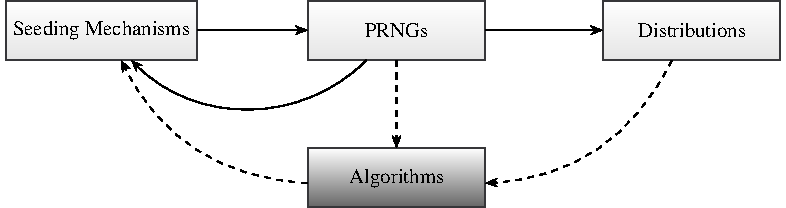
\includegraphics[width=\textwidth]{figures/api_parts.pdf}
      \end{figure}
      \begin{itemize}
        \pause\item PRNGs: MT19937, Xoroshiro128+, MSWS
        \pause\item real and integer uniform distributions
        \pause\item different seeding facilities
      \end{itemize}
    \end{frame}
  % section design (end)

  \section{Vectorization and SIMD Architectures} % (fold)
    \begin{frame}{SIMD Architecture}
      \begin{figure}
        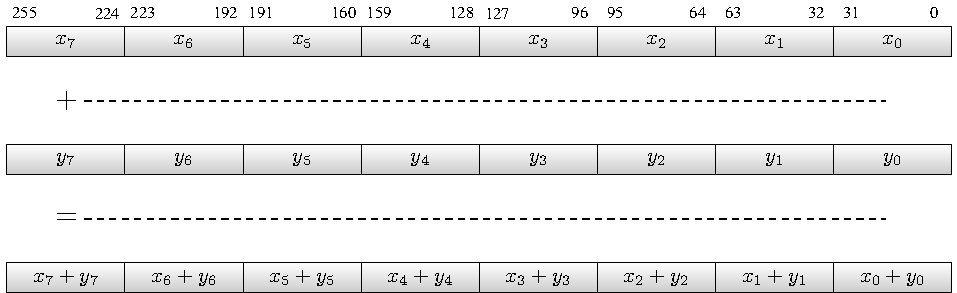
\includegraphics[width=0.8\textwidth]{figures/simd_vector_operations.pdf}
      \end{figure}
      \begin{itemize}
        \pause
        \item Single Instruction Multiple Data
        \pause
        \item processor contains vector registers multiple elements
        \pause
        \item processor operates on all values simultaneously
      \end{itemize}
    \end{frame}

    \begin{frame}{SIMD Implementations}
      Actual Hardware:
      \begin{itemize}
        \pause
        \item SSE, AVX and AVX512 instruction sets by Intel
        \pause
        \item Assembler Instructions $|$ Automatic Vectorization $|$ SIMD Intrinsics
      \end{itemize}
      \bigskip
      \pause
      Why should we (manually) vectorize PRNGs?
      \begin{itemize}
        \pause
        \item performance and speed
        \pause
        \item no automatic vectorization possible
        \pause
        \item external vectorized code needs random numbers
        \pause
        \item performance portability
        % \pause\item use full functionality of today's processors
        % \pause\item faster generation of numbers
        % \pause\item PRNGs are low-level, SIMD is low-level
      \end{itemize}
    \end{frame}

    % \begin{frame}{SIMD Architecture}
    %   What are conditions for good vectorization?
    %   \begin{itemize}
    %     \pause
    %     \item nearly no data dependencies
    %     \pause
    %     \item same processing pipeline
    %     \pause
    %     \item branchless execution
    %     \pause
    %     \item CPU-bound algorithms
    %   \end{itemize}
    % \end{frame}

    \begin{frame}{SIMD Example}
      \begin{figure}
        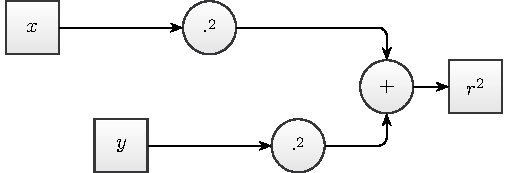
\includegraphics[width=0.5\textwidth]{figures/radius_operation.pdf}
      \end{figure}
      \begin{mybox}
        \[
          x,y\in\setReal, \qquad r^2 = x^2 + y^2
        \]
      \end{mybox}
    \end{frame}

    \begin{frame}{SIMD Example}
      \begin{figure}
        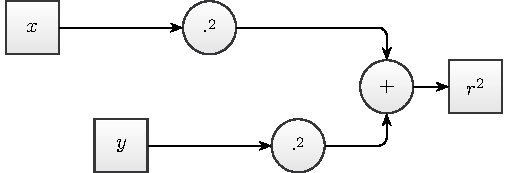
\includegraphics[scale=0.9]{figures/radius_operation.pdf}
      \end{figure}
    \end{frame}

    \begin{frame}{SIMD Example}
      \begin{figure}
        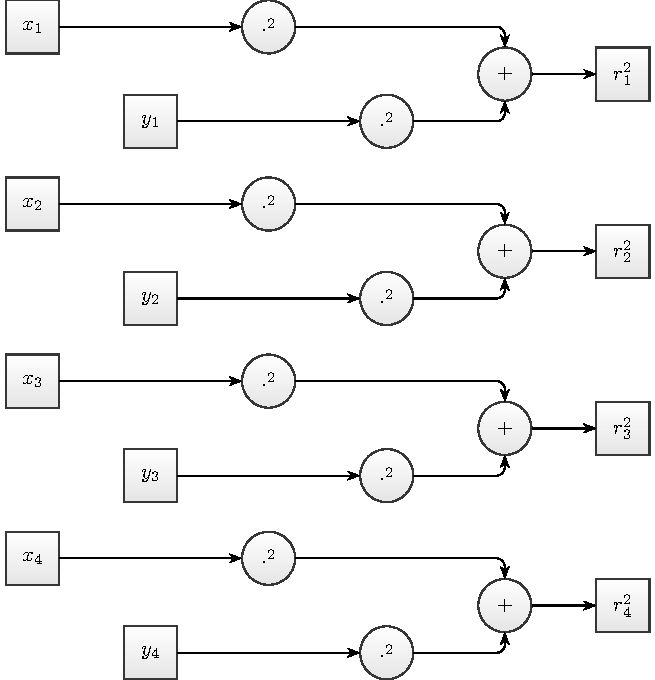
\includegraphics[scale=0.6]{figures/radius_operation_x4.pdf}
      \end{figure}
    \end{frame}

    \begin{frame}{SIMD Example}
      \begin{figure}
        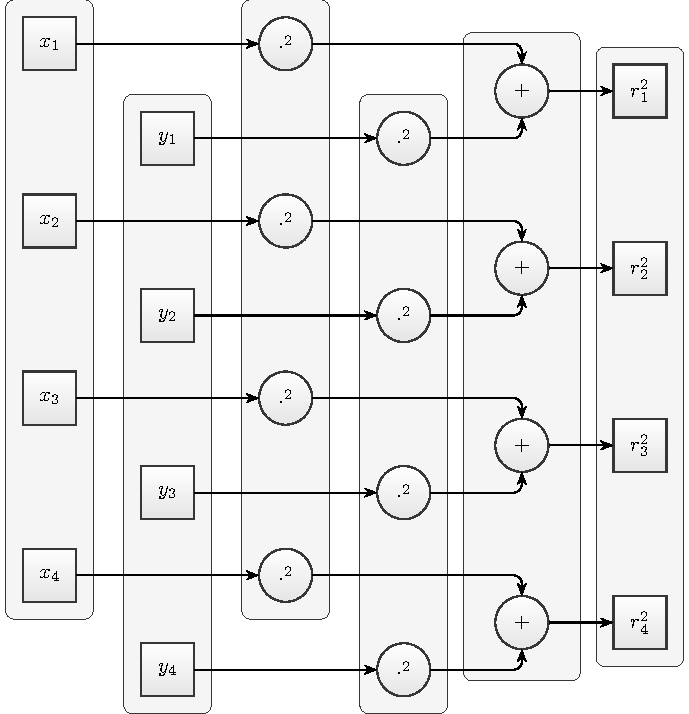
\includegraphics[scale=0.6]{figures/radius_operation_simd.pdf}
      \end{figure}
    \end{frame}

    % \begin{frame}{SIMD Example}
    %   % \begin{mybox}
    %     \begin{minipage}{0.48\textwidth}
    %     %   \begin{figure}
    %         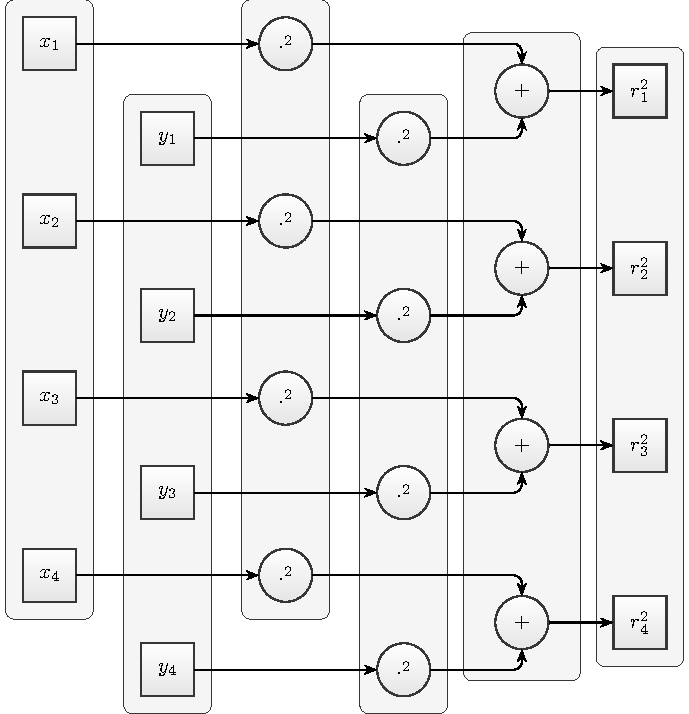
\includegraphics[scale=0.5]{figures/radius_operation_simd.pdf}
    %     %   \end{figure}
    %     \end{minipage}
    %     % \hfill\vrule\hfill
    %     \begin{minipage}[c]{0.50\textwidth}
    %       \begin{mybox}
    %         \inputCodeBlock{code/simd_example_avx.cpp}
    %       \end{mybox}
    %     \end{minipage}
    %   % \end{mybox}
    % \end{frame}

    % \begin{frame}{SIMD Example}
    %   \begin{mybox}
    %     \begin{minipage}{0.45\textwidth}
    %       \inputCodeBlock{code/simd_example_scalar.cpp}
    %     \end{minipage}
    %     \hfill\vrule\hfill
    %     \begin{minipage}{0.45\textwidth}
    %       \inputCodeBlock{code/simd_example_avx.cpp}
    %     \end{minipage}
    %   \end{mybox}
    % \end{frame}
  % section fundamentals_of_computer_architecture (end)

  \section{Xoroshiro128+} % (fold)
  \label{sec:implementation}
    % \subsection{Xoroshiro128+}
    \begin{frame}{Xoroshiro128+ Scheme}
      \begin{figure}
        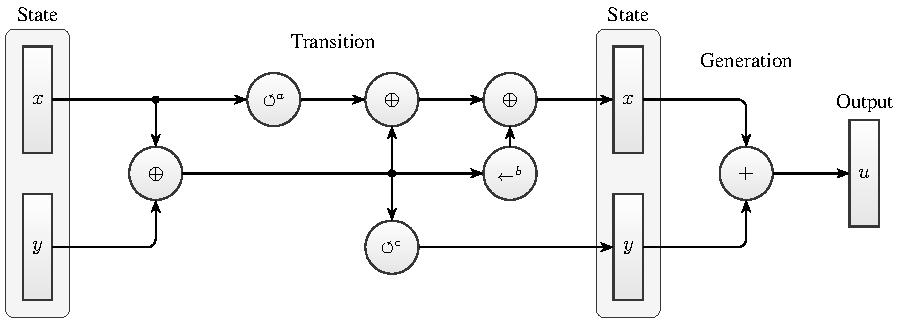
\includegraphics[width=0.8\textwidth]{figures/xrsr128p_scheme.pdf}
      \end{figure}
      \bigskip
      \begin{itemize}
        \pause
        \item scrambled linear PRNG
        \pause
        \item 128-bit state, 64-bit output
        \pause
        \item period: $2^{128}-1$
      \end{itemize}
    \end{frame}

    \begin{frame}{Xoroshiro128+ SIMD Scheme}
      \begin{figure}
        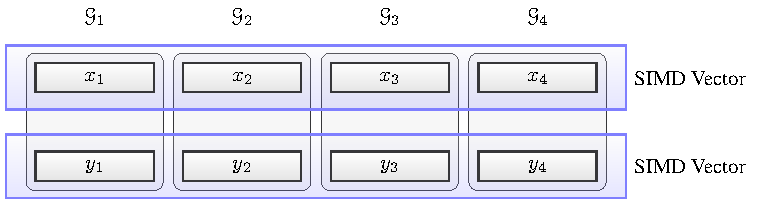
\includegraphics[width=0.9\textwidth]{figures/xrsr128p_vector_layout.pdf}
      \end{figure}
      \begin{itemize}
        \pause
        \item multiple instances of the same generator
        \pause
        \item seeding and parameter variations for multiple streams
        \pause
        \item four times more memory needed
      \end{itemize}
    \end{frame}

    % \subsection{MT19937}
    \section{Mersenne Twister MT19937}
    \begin{frame}{MT19937}
      \begin{figure}
        % 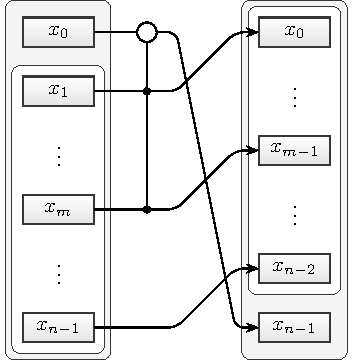
\includegraphics[width=0.25\textwidth]{figures/mt19937_transition_short.pdf}
        % \hfill
        % 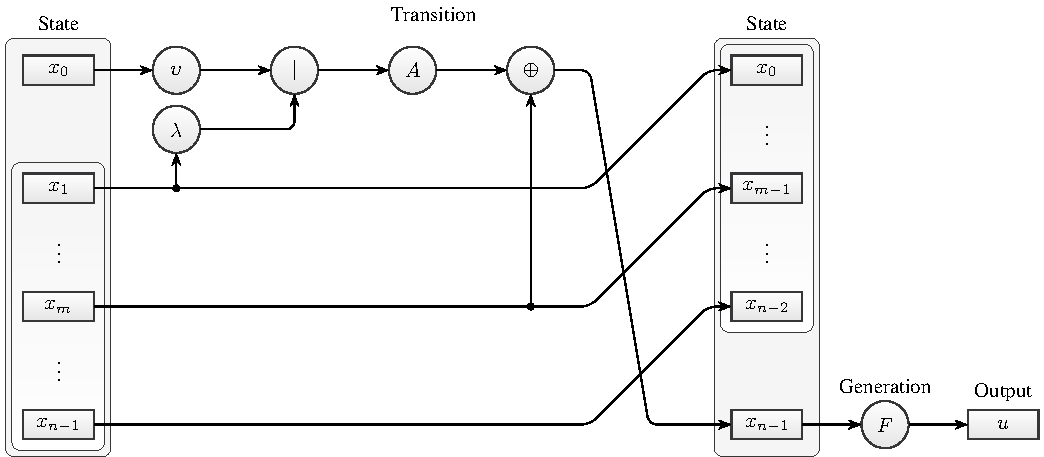
\includegraphics[width=0.637\textwidth]{figures/mt19937_scheme.pdf}
        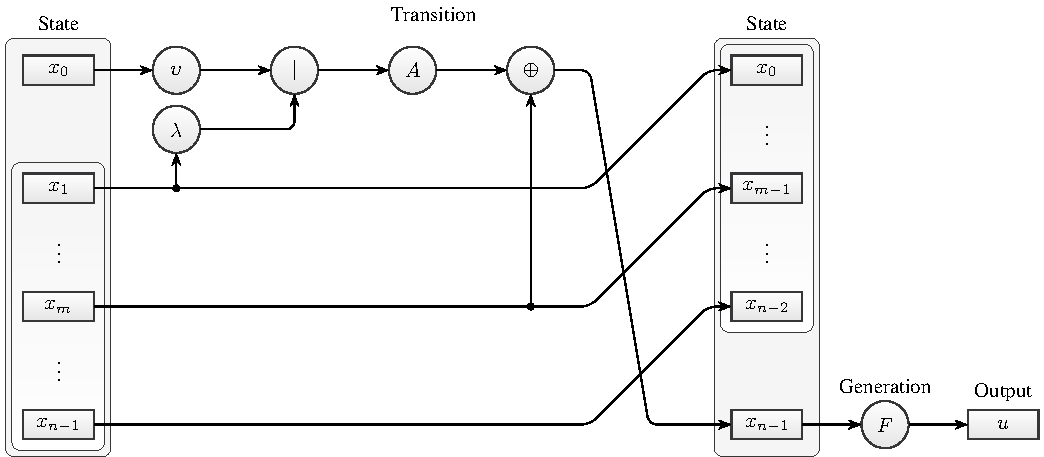
\includegraphics[width=0.72\textwidth]{figures/mt19937_scheme.pdf}
      \end{figure}
      \begin{itemize}
        \pause
        \item de-facto standard
        \pause
        \item linear PRNG
        \pause
        \item 19937-bit state, 32-bit output, $n=624$, $m=397$
      \end{itemize}
    \end{frame}

    \begin{frame}{MT19937}
      \begin{figure}
        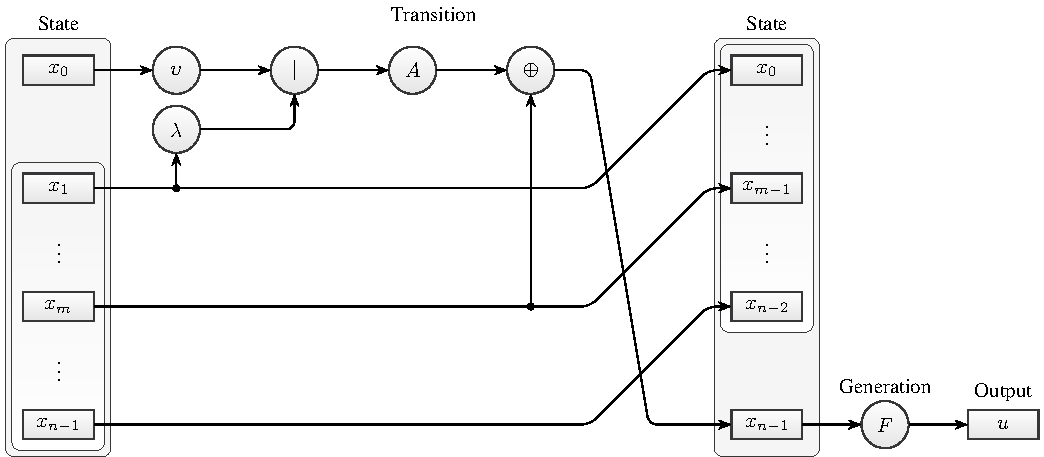
\includegraphics[width=0.72\textwidth]{figures/mt19937_scheme.pdf}
      \end{figure}
      \begin{itemize}
        \item period: $2^{19937}-1$
        \pause
        \item 623-dimensional equidistributed
        \pause
        \item vectorization of generation function analog to example
      \end{itemize}
    \end{frame}

    \begin{frame}{MT19937 Abbreviation}
      \begin{figure}
        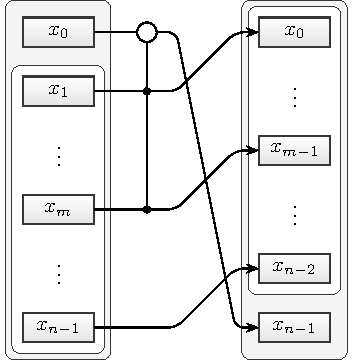
\includegraphics[width=0.25\textwidth]{figures/mt19937_transition_short.pdf}
        \hfill
        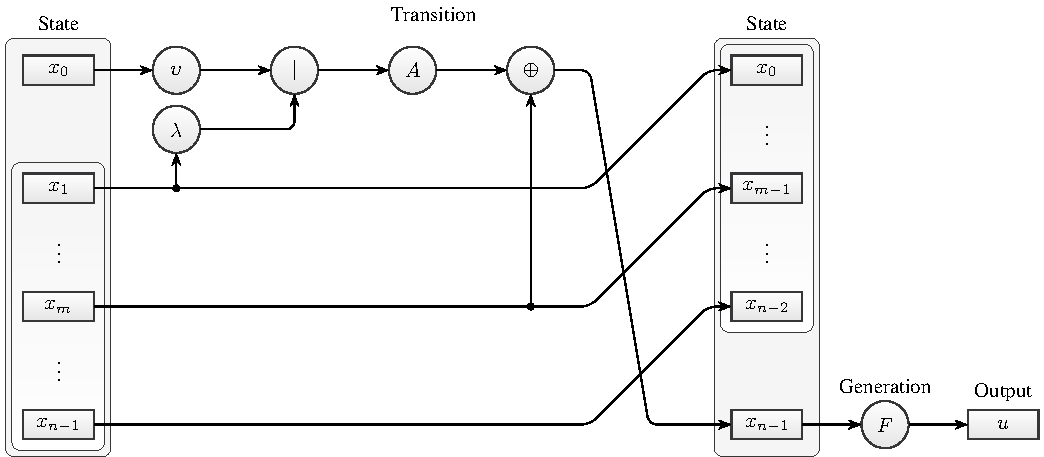
\includegraphics[width=0.637\textwidth]{figures/mt19937_scheme.pdf}
      \end{figure}
    \end{frame}

    \begin{frame}{MT19937 Scalar Loop Scheme}
      \begin{figure}
        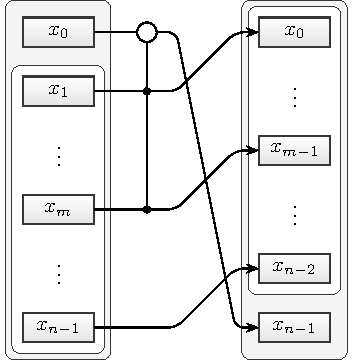
\includegraphics[width=0.25\textwidth]{figures/mt19937_transition_short.pdf}
        \hfill
        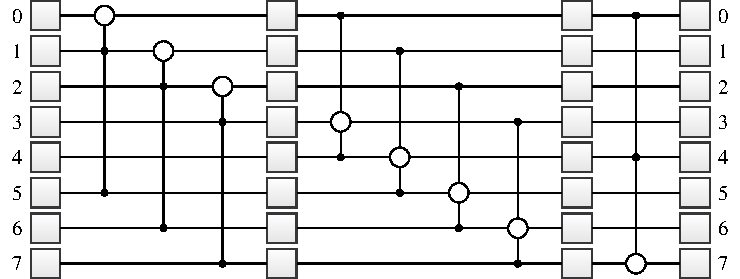
\includegraphics[width=0.7\textwidth]{figures/mt19937_loop_scheme.pdf}
      \end{figure}
      \begin{itemize}
        \pause
        \item moving all elements with one transition is inefficient
        \pause
        \item instead do $n$ transitions at once
        \pause
        \item example with $n=8$ and $m=5$
      \end{itemize}
    \end{frame}

    \begin{frame}{MT19937 SIMD Loop Scheme}
      \begin{figure}
        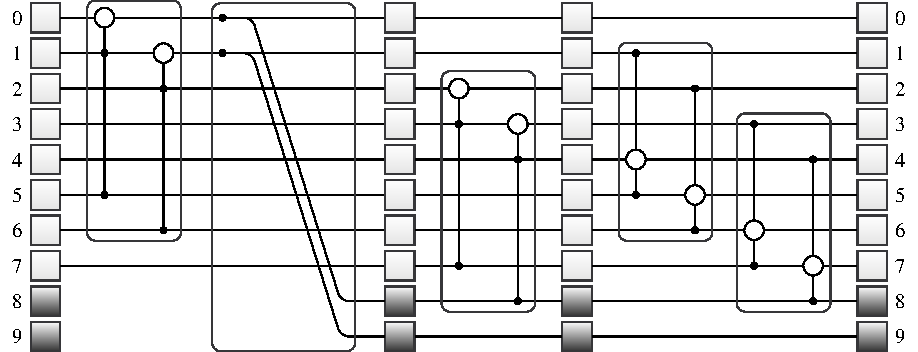
\includegraphics[width=0.8\textwidth]{figures/mt19937_vector_loop_scheme.pdf}
      \end{figure}
      \begin{itemize}
        \pause
        \item example: two-element-vector; reality: up to eight-element-vector
        \pause
        \item add vector-register-sized buffer at the end
        \pause
        \item copy generated head to the end and do the vectorized loop
      \end{itemize}
    \end{frame}

    \section{Uniform Distribution Functions}
    \begin{frame}{Real Uniform Distribution: Floating-Point Encoding}
      \begin{figure}
        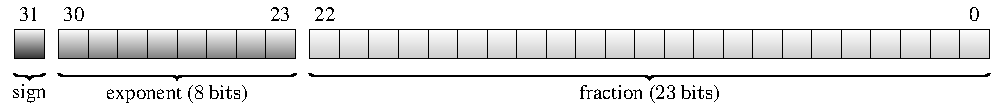
\includegraphics[width=0.95\textwidth]{figures/floating-point_encoding_single.pdf}
      \end{figure}
      \begin{mybox}
        \[
          x = (-1)^s \cdot m \cdot 2^{e - o}
        \]
      \end{mybox}
      \begin{itemize}
        \item IEEE 754
        \item we use only normalized numbers
      \end{itemize}
    \end{frame}

    \begin{frame}{Real Uniform Distribution}
      \begin{figure}
        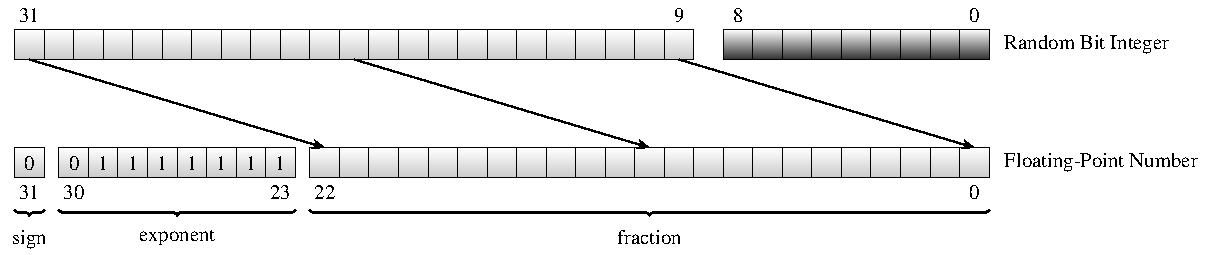
\includegraphics[width=0.95\textwidth]{figures/uniform_implementation_scheme.pdf}
      \end{figure}
      \begin{itemize}
        \pause
        \item get random integer
        \pause
        \item shift bits with highest entropy into fraction part
        \pause
        \item set sign and exponent to generate value in $[1,2)$
        \pause
        \item subtract one from result
      \end{itemize}
    \end{frame}

    \begin{frame}{Integer Uniform Distribution}
      \begin{itemize}
        \pause
        \item unbiased uniform integer algorithms should not be vectorized
        \pause
        \item use simple multiplication-based approximation
      \end{itemize}
      \bigskip
      \begin{mybox}
        \[
          x\in\setNatural_0,\ x < 2^{32},\qquad y = \floorBrackets{\frac{(b-a)\cdot x}{2^{32}}} + a
        \]
      \end{mybox}
      \bigskip
      \begin{itemize}
        \pause
        \item use 64-bit multiplication for 32-bit integers
        \pause
        \item bias can be neglected for typical simulations
      \end{itemize}
    \end{frame}
  % section implementation (end)

  \section{Evaluation and Results} % (fold)
  \label{sec:evaluation_and_results}
    \begin{frame}{Tests and Performance}
      \begin{itemize}
        \pause
        \item Consistency and Correctness: Unit Tests, API Tests, Examples
        \pause
        \item Statistical Performance: TestU01, dieharder
        \pause
        \item Performance: Filling a Cache, Monte Carlo π
      \end{itemize}
      \begin{figure}
        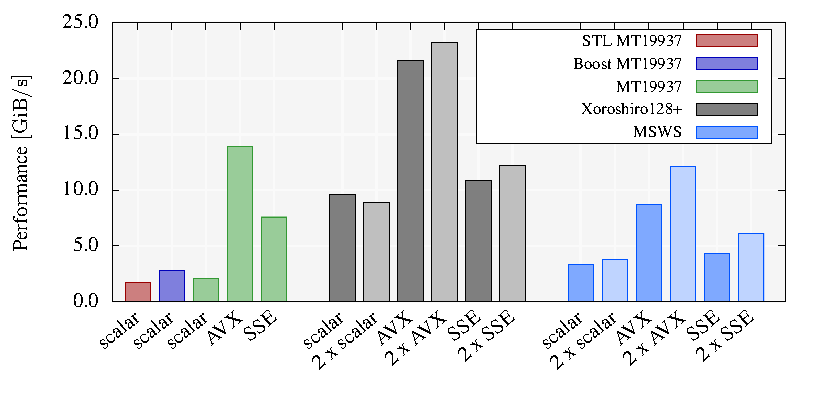
\includegraphics[width=0.6\textwidth]{figures/generation_desktop.pdf}
      \end{figure}
    \end{frame}

    \begin{frame}{Comparison to Intel MKL VSL and RNGAVXLIB}
      \begin{table}
        \caption{MT19937 Monte Carlo π Benchmark for $10^8$ Samples}
        \begin{tabular}{rrrr}
          \hline
          RNGAVXLIB & Intel MKL VSL & Cached AVX & Pure AVX \\
          \hline
          \hline
          $0.38\appendUnit{s}$ & $0.10\appendUnit{s}$ & $0.09\appendUnit{s}$ & $0.08\appendUnit{s}$ \\
          \hline
        \end{tabular}
      \end{table}
      \bigskip
      \begin{itemize}
        \pause
        \item pXart is faster in Monte Carlo π benchmark
        \pause
        \item scalar interface of RNGAVXLIB reduces performance
        \pause
        \item Intel MKL VSL always fills vector of data
        \pause
        \item benchmarks are biased
      \end{itemize}
    \end{frame}

    \begin{frame}{Comparison to Intel MKL VSL and RNGAVXLIB}
      \definecolor{cred}{rgb}{0.8, 0.1, 0.1}
      \definecolor{cgreen}{rgb}{0.1, 0.8, 0.1}
      \definecolor{bgc}{rgb}{0.9,0.9,0.9}
      \renewcommand{\checkmark}{\textcolor{cgreen}{\ding{52}}}
      \newcommand{\crossmark}{\textcolor{cred}{\ding{56}}}
      \begin{table}
        \begin{tabular}{lccc}
          \hline
          & pXart & RNGAVXLIB & Intel MKL VSL \\
          \hline
          \hline
          \rowcolor{bgc}
          Portable & \checkmark & \crossmark & \checkmark \\
          Good API & \checkmark & \crossmark & \crossmark \\
          \rowcolor{bgc}
          Open Source & \checkmark & \checkmark & \crossmark \\
          Documentation & \checkmark & \crossmark & \checkmark \\
          \rowcolor{bgc}
          Alternative Distributions & \crossmark & \checkmark & \checkmark \\
          AVX512 Support & \crossmark & \crossmark & \checkmark \\
          \hline
          \hline
          \rowcolor{bgc}
          Header-Only & \checkmark & \crossmark & \crossmark \\
          Build System Support & \checkmark & \crossmark & \crossmark \\
          % Dependency-Free & \checkmark & \checkmark & $\sim$ \\
          \hline
        \end{tabular}
      \end{table}
    \end{frame}
  % section evaluation_and_results (end)

  \section{Conclusions and Future Work} % (fold)
  \label{sec:conclusions}
    \begin{frame}{Conclusions}
      \begin{itemize}
        \pause\item photon simulation and path tracing
        \pause\item vectorized PRNGs speedup code even with caches
        \pause\item MT19937 or Xoroshiro128+?
      \end{itemize}
    \end{frame}
    \begin{frame}{Future Work}
      \begin{itemize}
        % \item more PRNGs, more Distributions, more Algorithms
        \pause\item alternative distributions
        \pause\item seeding mechanisms for thread support
        \pause\item AVX512 support
        \pause\item latency optimizations
        \pause\item application to real-world problems
        % \item C++20 support
        % \item wrap SIMD
      \end{itemize}
    \end{frame}
  % section conclusions (end)

  \begin{frame}
    \vfill
    \centering
    \begin{beamercolorbox}[sep=8pt,center,shadow=true,rounded=true]{title}
      \usebeamerfont{title}%
      Thank you for Your Attention!%
      \par%
    \end{beamercolorbox}
    \vfill
  \end{frame}

  \begin{frame}
      \frametitle{References}
      \tiny
      \begin{multicols}{2}
        \nocite{*}
        \bibliography{references}
      \end{multicols}
    \end{frame}

  \appendix

  \begin{frame}{Appendix: Pseudorandom Number Generator Concept}
    \begin{figure}
      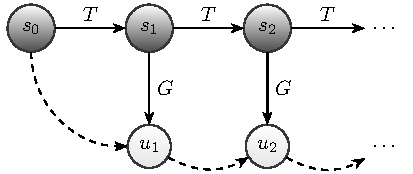
\includegraphics[width=0.5\textwidth]{figures/sequence_generation_scheme.pdf}
    \end{figure}
    \vfill
    \begin{mybox}
      \[
        s_0 \sim \mathscr{U}_S,\qquad
        u_1 \leftarrow \mathscr{G}(),\qquad
        u_2 \leftarrow \mathscr{G}(),\qquad
        u_3 \leftarrow \mathscr{G}(),\qquad \ldots
      \]
    \end{mybox}
  \end{frame}

  \begin{frame}{Appendix: Pseudorandom Number Generator Example}
    \begin{figure}
      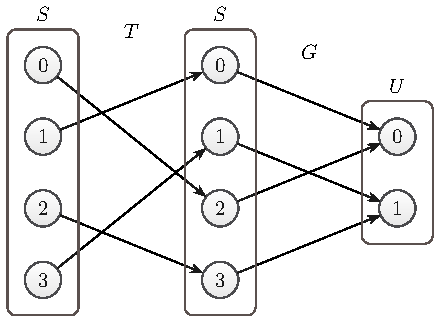
\includegraphics[width=0.45\textwidth]{figures/prng_example.pdf}
    \end{figure}
    \begin{mybox}
      \[
        s_0 \define 0, \qquad
        (s_n) = \overline{2310}, \qquad
        (u_n) = \overline{0110}
      \]
    \end{mybox}
  \end{frame}

  \begin{frame}{Appendix: Pseudorandom Number Generator Example}
    \begin{figure}
      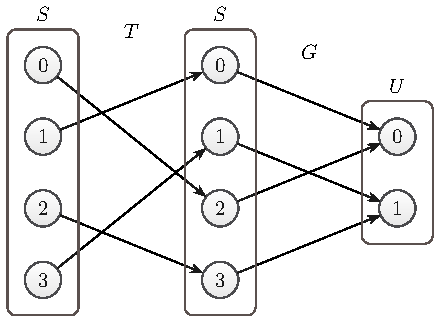
\includegraphics[width=0.45\textwidth]{figures/prng_example.pdf}
    \end{figure}
    \begin{itemize}
      \item construction of \enquote{good} PRNG is difficult
      \pause
      \item pseudorandom number sequences will be periodic
    \end{itemize}
  \end{frame}

  \begin{frame}{Appendix: pXart Usage in C++}
    \hspace{5em}
    \begin{minipage}[c]{0.8\textwidth}
      \inputCodeBlock{code/api.cpp}
    \end{minipage}
  \end{frame}

  \begin{frame}{Appendix: Computation of π}
    \begin{figure}
      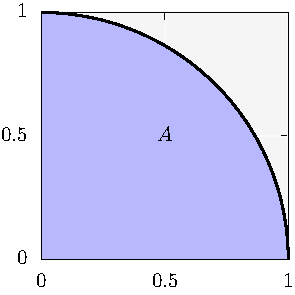
\includegraphics[width=0.3\textwidth]{plots/monte_carlo_pi_circle.pdf}
    \end{figure}
    \begin{mybox}
      \[
        A = \frac{π}{4}, \qquad \hat{π} = \frac{4 N_A}{N}
      \]
    \end{mybox}
  \end{frame}

  \begin{frame}{Appendix: Computation of π}
    \begin{figure}
      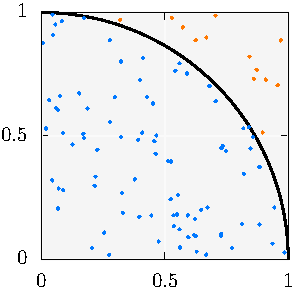
\includegraphics[width=0.3\textwidth]{figures/monte_carlo_pi_100_87.pdf}
    \end{figure}
    \begin{mybox}
      \[
        A = \frac{π}{4}, \qquad \hat{π} = \frac{4 N_A}{N} = \frac{4 \cdot 87}{100} = 3.48
      \]
    \end{mybox}
  \end{frame}

  \begin{frame}{Appendix: Computation of π}
    \begin{figure}
      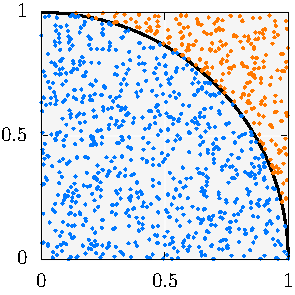
\includegraphics[width=0.3\textwidth]{figures/monte_carlo_pi_1000_765.pdf}
    \end{figure}
    \begin{mybox}
      \[
        A = \frac{π}{4}, \qquad \hat{π} = \frac{4 N_A}{N} = \frac{4 \cdot 765}{1000} = 3.06
      \]
    \end{mybox}
  \end{frame}

  \begin{frame}{Appendix: Computation of π}
    \begin{figure}
      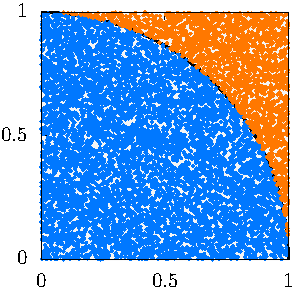
\includegraphics[width=0.3\textwidth]{figures/monte_carlo_pi_10000_7856.pdf}
    \end{figure}
    \begin{mybox}
      \[
        A = \frac{π}{4}, \qquad \hat{π} = \frac{4 N_A}{N} = \frac{4 \cdot 7856}{10000} = 3.1424
      \]
    \end{mybox}
  \end{frame}

  \begin{frame}{Appendix: Example Usage}
    \hspace{8em}
    \begin{minipage}[c]{0.7\textwidth}
      \inputCodeBlock{code/monte_carlo_pi.cpp}
    \end{minipage}
  \end{frame}

  \begin{frame}{Appendix: Processor}
    \begin{figure}
      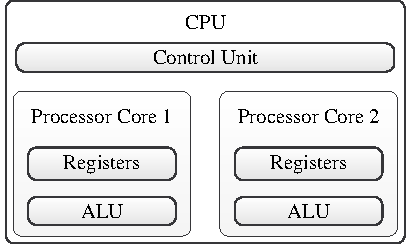
\includegraphics[height=0.5\textheight]{figures/cpu_components.pdf}
    \end{figure}
  \end{frame}

  \begin{frame}{Appendix: Memory Hierarchy}
    \begin{figure}
      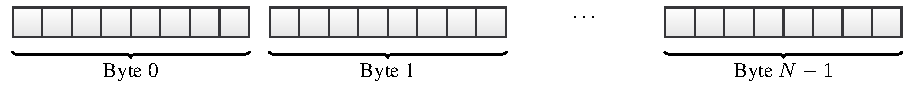
\includegraphics[width=0.95\textwidth]{figures/memory.pdf}
    \end{figure}
    \begin{figure}
      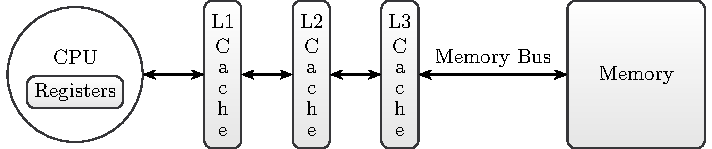
\includegraphics[width=0.95\textwidth]{figures/memory_hierarchy.pdf}
    \end{figure}
  \end{frame}

  \begin{frame}{Appendix: MT19937 SIMD Leap Frogging}
    \begin{figure}
      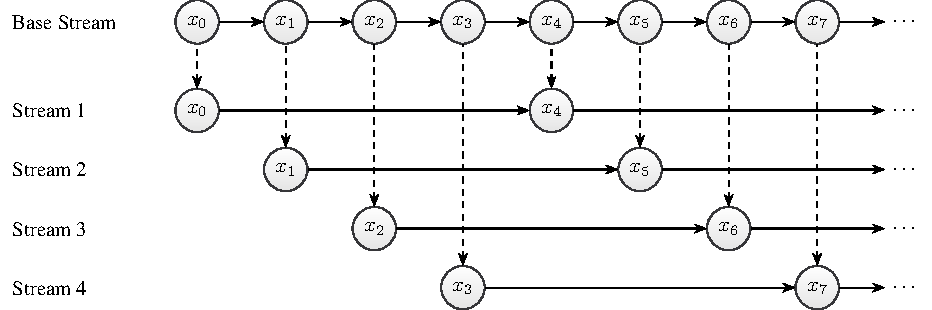
\includegraphics[width=0.9\textwidth]{figures/leapfrogging_multiple_streams.pdf}
    \end{figure}
    \begin{itemize}
      \item vectorized generator will give same output as scalar one, only faster
    \end{itemize}
  \end{frame}

  \begin{frame}{Appendix: MT19937 Speed-Up Monte Carlo π}
    \begin{figure}
      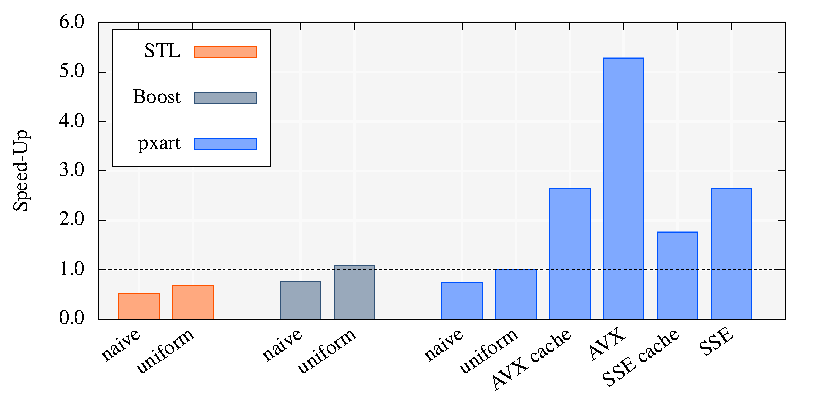
\includegraphics[width=0.6\textwidth]{figures/monte_carlo_pi_desktop_mt19937.pdf}\\
    \end{figure}
  \end{frame}

  \begin{frame}{Appendix: Xoroshiro128+ Speed-Up Monte Carlo π}
    \begin{figure}
      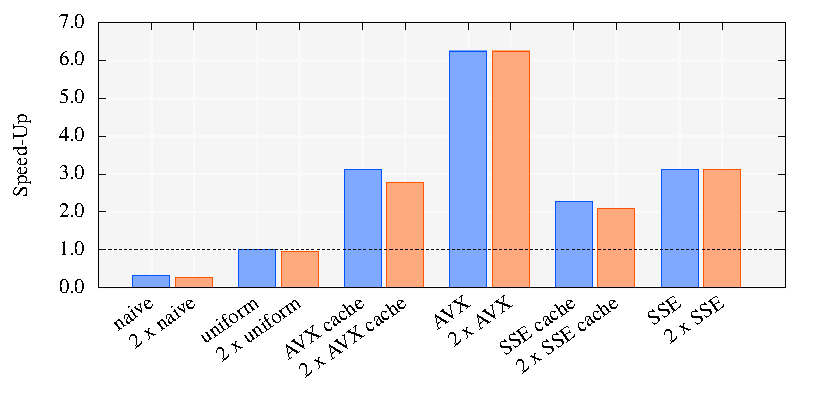
\includegraphics[width=0.6\textwidth]{figures/monte_carlo_pi_desktop_xrsr128p.pdf}
    \end{figure}
  \end{frame}
\end{document}